\documentclass[11pt,a4paper]{article}

%% ── Core Layout and Geometry ────────────────────────────────────────────────
\usepackage[utf8]{inputenc}
\usepackage[T1]{fontenc}
\usepackage[margin=1in]{geometry}
\usepackage{microtype}
\usepackage{setspace}
\onehalfspacing

%% ── Typography: Professional Math and Text ─────────────────────────────────
\usepackage{mathptmx}
\usepackage{amsmath,amssymb,amsfonts}

%% ── Graphics, Tables, and Formatting ───────────────────────────────────────
\usepackage{graphicx}
\usepackage{booktabs}
\usepackage{multirow}
\usepackage{tabularx}
\usepackage{array}
\usepackage{siunitx}
\usepackage{xcolor}
\usepackage{url}
\usepackage{caption}
\usepackage{subcaption}

\captionsetup{
  font=small,
  labelfont=bf,
  justification=centering,
  skip=6pt
}

%% ── Headings Formatting ────────────────────────────────────────────────────
\usepackage{titlesec}
\titleformat{\section}{\large\bfseries}{\thesection}{0.75em}{}
\titlespacing*{\section}{0pt}{14pt}{6pt}
\titleformat{\subsection}{\normalsize\bfseries}{\thesubsection}{0.75em}{}
\titlespacing*{\subsection}{0pt}{10pt}{4pt}
\titleformat{\subsubsection}{\normalsize\itshape}{\thesubsubsection}{0.75em}{}
\titlespacing*{\subsubsection}{0pt}{8pt}{3pt}

%% ── Hyperlinks ─────────────────────────────────────────────────────────────
\usepackage{hyperref}
\hypersetup{
  colorlinks=true,
  linkcolor=blue!75!black,
  citecolor=blue!75!black,
  urlcolor=blue!75!black
}

%% ── Citations & Bibliography ───────────────────────────────────────────────
\usepackage[numbers,sort&compress]{natbib}
\setlength{\bibhang}{0.35in}

%% ── Mathematical Notation Shortcuts ────────────────────────────────────────
\newcommand{\yt}{y_t}
\newcommand{\yh}{\hat{y}}
\newcommand{\persistence}{\hat{y}_{t+h} = y_t}

%% ── Title Block ────────────────────────────────────────────────────────────
\title{%
  \Large\bfseries Benchmarking Supervised Machine Learning for Next-Day Air Quality Index Forecasting in Gujarat: \\
  An Empirical Audit of Data Leakage and a Multi-City Evaluation
}

\author{%
  \textbf{Pratham Dakshay Khatri}
}

\date{November 2026}

%% ════════════════════════════════════════════════════════════════════════════
\begin{document}
\maketitle

%% ── Abstract ────────────────────────────────────────────────────────────────
\begin{abstract}
\noindent
Short-term Air Quality Index (AQI) forecasting is vital for public health advisories in industrialising regions such as Gujarat, India. Regional studies routinely report high accuracy ($R^2 > 0.80$, often $> 0.95$), yet these results stem from \emph{concurrent input leakage} (same-day pollutants predicting same-day AQI) and \emph{random-split autocorrelation leakage}. We audit these mechanisms across five Gujarat cities (Ahmedabad, Gandhinagar, Ankleshwar, Vapi, Surat) and coastal Chennai using CPCB records (2015--2023) under Setup~A (random, concurrent), Setup~B (chronological, concurrent), and Setup~C (rolling-origin, lagged). In Ahmedabad, Random Forest drops from $R^2 = \mathbf{0.815}$ ($\text{MAE}=18.50$) under Setup~A to $\mathbf{0.015}$ ($\text{MAE}=30.49$) under Setup~B, consistent with a March--May 2020 regime and pollutant-missingness shift; on 141 non-lockdown days, concurrent Setup~B ($\text{MAE}=18.01$) still sharply outperforms like-for-like lagged Setup~C ($\text{MAE}=39.33$), confirming large concurrent-input inflation. Under leak-free Setup~C ($h=1$), no ML model significantly beats Persistence ($\hat{y}_{t+1}=y_t$) in five of six cities ($p > 0.05$), and in Vapi Persistence is superior to all complex models ($p \le 0.003$). Simple ARIMA(1,0,0) beats Persistence in Gandhinagar ($p=0.00045$), Surat ($p=0.011$), and Chennai ($p=0.0035$). In coastal Chennai, ML achieves nominally significant $h=1$ skill ($+11.5\%$ RF, $p=0.002$; fails Bonferroni under $k=0$, though XGBoost would survive under $k=3$ at $p=0.00075$), but RF is sensitive to dropping imputed pollutant lags ($p=0.087$). At $h=3$, Chennai Ridge and XGBoost outperform both Persistence ($p \le 0.0006$) and ARIMA(1,0,0) ($p \le 0.0001$). We release our complete codebase, datasets, and prediction ledgers.
\end{abstract}

\vspace{0.5em}
\noindent\textbf{Keywords:} Air Quality Index, Data Leakage, Time-Series Forecasting, Rolling-Origin Evaluation, Persistence Baseline, Diebold-Mariano Test, Gujarat.

%% ════════════════════════════════════════════════════════════════════════════
\section{Introduction}
\label{sec:intro}

Ambient air pollution is among the most pressing environmental health challenges in modern India, contributing to an estimated 1.67 million premature deaths in 2019 \cite{pandey2021} and imposing substantial socio-economic burdens. While national monitoring efforts have expanded dramatically under the National Clean Air Programme (NCAP), reliable predictive capabilities remain vital. Robust short-range forecasts of the daily Air Quality Index (AQI) afford municipal authorities, environmental regulators, and vulnerable populations actionable lead time to implement emergency interventions, regulate industrial emissions, and restrict vehicular circulation.

Gujarat, located along India's western industrial corridor, represents a critical yet under-studied theatre for atmospheric modeling. Hosting vast petrochemical complexes, chemical manufacturing zones, and rapidly expanding urban centres (notably Ahmedabad, Surat, Ankleshwar, and Vapi), Gujarat regularly records extreme concentrations of respirable particulate matter ($PM_{2.5}, PM_{10}$) and toxic gaseous pollutants ($SO_2, NO_2, CO$). In contrast to the National Capital Region (NCR) around Delhi, which has received extensive analytical attention, empirical machine learning research focused specifically on Gujarat's distinct geographical and industrial micro-climates remains sparse.

Over the past decade, a surge of applied machine learning literature has investigated urban AQI prediction across Indian municipalities. Authors have deployed linear estimators, support vector machines, Random Forests, Gradient Boosted Decision Trees (XGBoost, LightGBM, CatBoost), and diverse deep learning architectures (e.g., LSTM, GRU). These publications routinely report coefficients of determination ($R^2$) exceeding $0.80$ to $0.99$, concluding that nonlinear machine learning has effectively solved urban air quality forecasting \cite{maltare2023}\cite{sidhu2024}\cite{mishra2025}\cite{jayapradha2025}\cite{chauhan2026}.

In this paper, we argue that these reported results are heavily inflated by methodological flaws in experimental design. Specifically, two systematic modes of data leakage pervade published studies:

\paragraph{Concurrent Input Leakage (Nowcasting vs. Forecasting Conflation)}
The Central Pollution Control Board (CPCB) prescribes the official daily AQI as the non-linear algebraic supremum across criteria pollutant sub-indices:
\begin{equation}
  \text{AQI}_t = \max_{p \in \mathcal{P}} I_p(C_{p,t})
  \label{eq:cpcb_aqi}
\end{equation}
where $\mathcal{P} = \{PM_{2.5}, PM_{10}, NO_2, SO_2, CO, O_3, NH_3\}$ is the set of monitored criteria pollutants, $C_{p,t}$ is the daily mean concentration of pollutant $p$ on calendar day $t$ (a 24-hour mean for most pollutants; CPCB uses an 8-hour rolling average for CO and O$_3$), and $I_p(C_{p,t})$ is the piecewise-linear sub-index conversion function specified by Indian regulatory guidelines. Numerous applied studies train models where concurrent pollutant concentrations $\{C_{p,t}\}_{p \in \mathcal{P}}$ serve as independent input features to predict that same day's aggregate index $\text{AQI}_t$ \cite{sidhu2024}\cite{mishra2025}\cite{jayapradha2025}\cite{chauhan2026}. Because same-day pollutant concentrations cannot be observed hours or days in advance, this configuration does not represent operational forecasting; it performs static algebraic reconstruction or nowcasting. (In our own Setup~A, concurrent inputs reconstruct the target with $R^2 = 0.815$ rather than $1.0$, likely because the target is the official CPCB daily bulletin index whereas the pollutant inputs come from a separate station-level Kaggle archive.)

\paragraph{Random-Split Autocorrelation Leakage}
Urban daily AQI series exhibit intense temporal persistence and first-order autocorrelation ($\rho_1 \approx 0.75$ in Ahmedabad, above $0.83$ in Ankleshwar and Gandhinagar, and $0.90$ in Vapi).\footnote{Computed directly from the processed Parquet files via \texttt{pandas.Series.autocorr(lag=1)} on valid (non-NaN) AQI observations: Ahmedabad 0.753, Ankleshwar 0.836, Chennai 0.704, Gandhinagar 0.834, Surat 0.710, Vapi 0.901.} When datasets are partitioned using random train-test splitting (e.g., standard random 80/20 cross-validation), adjacent temporal observations ($t-1$ and $t+1$) invariably enter the training partition while day $t$ is placed in the test partition. Because adjacent days share nearly identical meteorological and atmospheric states, the model interpolates between proximal training points rather than projecting forward in time. This provides artificial predictive cues that collapse completely in deployment.

Although the pitfalls of evaluating time-series predictors with shuffled cross-validation have been examined in the forecasting literature \cite{bergmeir2012}\cite{cerqueira2020}, and leakage in predictive modelling has been formalised more broadly \cite{kaufman2012}, their practical effect on Indian AQI studies has not been systematically audited. Furthermore, published studies rarely evaluate simple heuristic benchmarks -- such as the naive Persistence forecaster ($\hat{y}_{t+1} = y_t$) -- or conduct formal statistical hypothesis testing (e.g., the Diebold-Mariano test \cite{diebold1995}) to establish whether machine learning models provide statistically verifiable skill over naive inertia.

\paragraph{Contributions.}
To address these deficiencies and establish rigorous benchmarks, this study delivers three primary contributions:
\begin{enumerate}
  \item \textbf{Empirical Quantification of Leakage Inflation:} We design three nested, controlled evaluation setups (Setups~A, B, and C) applied to municipal series, measuring the inflation associated with concurrent inputs, random train-test partitioning, and temporal distribution shifts.
  \item \textbf{Leak-Free Multi-City Benchmark for Gujarat:} To our knowledge, this is the first leak-free, persistence-benchmarked multi-city evaluation for Gujarat. We implement a strict rolling-origin expanding-window evaluation across five major Gujarat industrial and urban centres (Ahmedabad, Gandhinagar, Ankleshwar, Vapi, Surat) alongside Chennai as a maritime comparative anchor. We evaluate next-day ($h=1$) and three-day ($h=3$) lead times, pairing error distributions with 95\% moving block-bootstrap confidence intervals and Diebold-Mariano significance testing against Persistence.
  \item \textbf{Complete Open-Source Reproducibility Framework:} We release a fully modularised, tested Python package, verified dataset manifests with SHA-256 integrity checksums, and the 138 primary out-of-sample prediction trajectories (supplemented by classical baseline and sensitivity scripts), allowing the entire empirical pipeline to be executed via a single command.
\end{enumerate}

The remainder of this article is organized as follows: Section~\ref{sec:related} reviews related work and methodological pitfalls. Section~\ref{sec:data} details data curation, sensor range validation, and city qualification. Section~\ref{sec:method} formalises the evaluation protocols, leakage guards, candidate forecasters, and hypothesis testing framework. Section~\ref{sec:results} presents the empirical results. Section~\ref{sec:discussion} discusses meteorological mechanisms, practical implications, and limitations. Section~\ref{sec:conclusion} concludes.


%% ════════════════════════════════════════════════════════════════════════════
\section{Related Work}
\label{sec:related}

\subsection{Machine Learning for Air Quality Modeling in India}
The application of predictive algorithms to air pollution across Indian metropolitan centres has expanded rapidly. Urban air quality management in India has been reviewed extensively \cite{gulia2015}. Early forecasting studies relied primarily on classical statistical techniques such as autoregressive integrated moving average (ARIMA) models and multiple linear regression. With the public dissemination of continuous ambient air quality monitoring station (CAAQMS) records by the CPCB, researchers transitioned to nonlinear machine learning and deep learning algorithms.

In Gujarat, Maltare and Vahora~\cite{maltare2023} evaluated SARIMA, SVM, and LSTM on Ahmedabad (2015--2021), reporting $R^2 = 0.9989$ for SVM-RBF and $R^2 = 0.951$ for LSTM without specifying a chronological validation split or benchmarking against persistence. At the state level, Advitha et al.~\cite{advitha2024} applied Random Forest and XGBoost to seven Gujarat cities (including Ahmedabad, Ankleshwar, Surat, and Vapi), reporting $R^2 = 98.87\%$ and $98.27\%$ respectively for predicting the calculated AQI from $\text{PM}_{2.5}$, $\text{PM}_{10}$, $\text{SO}_2$, and $\text{NO}_x$ concentrations, without describing a train--test split or a persistence baseline; in their own correlation analysis the calculated AQI is perfectly correlated with $\text{PM}_{10}$ ($r = 1.00$), consistent with an AQI computed deterministically from the model inputs. Surat has also been studied with ARIMA \cite{mahendra2023}. Across broader Indian regions, Sidhu et al.~\cite{sidhu2024} applied CatBoost, XGBoost, and Random Forest across 22 stations in Delhi, Haryana, and Punjab, reporting $R^2 \approx 1.0$ when feeding eight same-day pollutants to predict same-day AQI. Similarly, Chauhan and Sutaria~\cite{chauhan2026} compared SVM, GBM, and XGBoost across six Indian metropolitan cities (including Ahmedabad) using concurrent hourly pollutant inputs, while Mishra et al.~\cite{mishra2025} reported $R^2 = 0.961\text{--}0.9985$ across South Indian cities using a randomly ordered 80:20 split with seven same-day pollutants. Jayapradha et al.~\cite{jayapradha2025} reported $R^2 = 0.948$ for a hybrid LSTM--RF--XGBoost model on multi-city Kaggle records where both same-day pollutants and the derived AQI category (\texttt{AQI\_Bucket}) ranked among top features, and Chakraborty and Shanthi~\cite{chakraborty2026} (a preprint) reported GRU $R^2 = 0.9886$ using AQI-average features whose windows include the current timestep ($i=0$), which risks target leakage if $\text{AQI}_t$ is the target (the target is not explicitly stated). By contrast, Singh et al.~\cite{singh2025} candidly documented severe generalization collapse in pan-India $\text{PM}_{2.5}$ modeling (Random Forest train $R^2 = 0.99$ versus test $R^2 = 0.35$). Meanwhile, Malhotra et al.~\cite{malhotra2024} systematically surveyed AI-based air pollution prediction studies, with an emphasis on India, cataloging validation schemes (e.g., $k$-fold, 70/30) without auditing data leakage.

Close examination shows that several of these studies \cite{sidhu2024}\cite{mishra2025}\cite{jayapradha2025}\cite{chauhan2026}\cite{advitha2024} use concurrent pollutant inputs to predict same-day AQI, and some also use random train-test splits \cite{mishra2025}; for others \cite{maltare2023}\cite{advitha2024}\cite{chakraborty2026}, the validation design is unreported or ambiguous. These are the two leakage mechanisms described in Section~\ref{sec:intro}.

\subsection{Temporal Data Leakage and Validation Protocols}
Data leakage occurs when training data inadvertently incorporates information that would be unavailable at inference time, inducing severe optimistic bias \cite{kaufman2012}. In temporal and spatial machine learning, leakage typically arises through lookahead bias (conditioning on future events) or serial dependency exploitation \cite{bergmeir2012}.

Cerqueira et al.~\cite{cerqueira2020} conducted an extensive comparative benchmark of performance-estimation methods for time series, finding that standard random $k$-fold cross-validation produces systematically over-optimistic estimates for non-stationary data, whereas out-of-sample holdout and prequential (rolling-origin) methods yield estimates that mirror real-world generalization. The severity of this distortion in applied benchmarks is further documented by Albelali and Ahmed~\cite{albelali2025}, who showed that LSTM models trained with cross-validation on sliding windows (built before partitioning) overestimate performance by up to 20.5\% in RMSE, and by Garc{\'i}a Crespi et al.~\cite{garciacrespi2026}, who demonstrated using daily PM$_{10}$ data from Elche, Spain that rolling-origin validation \emph{reverses model rankings} relative to a simple persistence baseline when compared to static hold-out splits. Outside India, Xie and Tummala~\cite{xie2025} benchmarked boosting algorithms across healthcare, environmental, and energy sensor data and found that random $k$-fold cross-validation on Beijing $\text{PM}_{2.5}$ inflated $R^2$ to roughly $0.87$, whereas chronological validation produced negative $R^2$ values. Similarly, Ayus et al.~\cite{ayus2023} reported that XGBoost outperformed deep learning across 10 Chinese cities based on a random 80/20 split with concurrent pollutant inputs, underscoring how pervasive unvalidated splitting remains in atmospheric ML.

\subsection{Persistence Benchmarking and the Forecast Skill Metric}
A fundamental principle of meteorological forecast verification is that any proposed prognostic model must be evaluated against standard climatological and persistence benchmarks \cite{murphy1992}\cite{jolliffe2012}. In strongly autocorrelated processes, the naive Persistence forecaster ($\hat{y}_{t+h} = y_t$) represents a formidable obstacle, particularly at short forecast horizons ($h=1$).

Time-aware evaluation has begun to appear for Indian cities more broadly: Goetzinger et al.~\cite{goetzinger2026} used leakage-safe lag features with a strictly chronological holdout, and Dar et al.~\cite{dar2025} used rolling-origin validation with naive seasonal baselines across ten cities. Most directly relevant to our study, Abidha et al.~\cite{abidha2026} conducted a leakage-aware case study for Chennai (2018--2024), demonstrating that same-day pollutant inputs were near-exact linear rescalings of AQI ($r > 0.9999$); once concurrent inputs were removed, reported $R^2$ collapsed from $1.0$ to $\approx 0.52$, nearly matched by naive Persistence ($R^2 = 0.475$, MAE $= 12.4$). Standard forecast-verification practice recommends reporting skill relative to a reference forecast such as persistence \cite{murphy1992}\cite{jolliffe2012}:
\begin{equation}
  \text{Skill} = 1 - \frac{\text{MAE}_{\text{model}}}{\text{MAE}_{\text{persistence}}}
  \label{eq:skill_def}
\end{equation}
where positive values signify genuine predictive value beyond inertial extrapolation. Extending Abidha et al.~\cite{abidha2026}, our study provides, to our knowledge, the first leak-free, persistence-benchmarked multi-city evaluation for Gujarat (including the industrial corridors of Surat, Vapi, and Ankleshwar, for which we are not aware of prior persistence-referenced evaluation), isolates random-split versus concurrent-input inflation via nested Setups A, B, and C, evaluates multi-day horizon decay ($h=1$ vs.\ $h=3$), and conducts formal Diebold-Mariano hypothesis testing \cite{diebold1995}.


%% ════════════════════════════════════════════════════════════════════════════
\section{Data and Preprocessing}
\label{sec:data}

\subsection{Data Sources and Provenance}
We integrate two official, open data repositories published under the statutory framework of India's CPCB:
\begin{enumerate}
  \item \textbf{CPCB Daily Air Quality Bulletins (2015--2023):} Official 4:00~PM bulletin reports published daily across all monitored municipal centres, archived on Zenodo (DOI: \href{https://doi.org/10.5281/zenodo.11146316}{10.5281/zenodo.11146316}; 299,974 records). Each bulletin reports the official municipal ``Index Value'', calculated according to CPCB guidelines based on active CAAQMS stations. This official index forms our primary target variable $\yt$.
  \item \textbf{CPCB Station Concentrations (Kaggle CAAQMS Archive):} Daily ambient concentration measurements for the seven criteria pollutants ($PM_{2.5}, PM_{10}, NO_2, SO_2, CO, O_3, NH_3$) spanning 2015--2020. Where station-aggregated AQI values diverged from official bulletins due to unbounded sub-index equations exceeding the theoretical maximum of 500, the official bulletin figure was enforced as the authoritative ground truth.
\end{enumerate}

\subsection{City Qualification and Regional Scope}
To evaluate geographical generalization, six municipal centres were qualified based on temporal continuity, data density, and industrial relevance. Table~\ref{tab:city_qualification} details the qualified cities, monitoring intervals, record counts, and assigned experimental roles.

\input{../results/tables/table1_qual.tex}

Ahmedabad and Chennai satisfy the longest historical continuity ($n = 3{,}167$ calendar days) and possess concurrent criteria pollutant measurements, qualifying for all three comparative setups (A, B, and C). Ahmedabad represents inland semi-arid western India, whereas Chennai serves as a maritime southern comparative anchor. Gandhinagar, Ankleshwar, and Vapi qualify from 2019 onward based on official CPCB daily bulletins. Surat, where CAAQMS stations first appear in the CPCB bulletin archive in late 2021 ($n = 423$ bulletin days; 327 valid observations with non-missing AQI), serves as a thin-data sensitivity evaluation. (The precise commissioning date of Surat's CAAQMS network is not formally documented in the publicly available CPCB technical reports; we infer it from the first occurrence of valid Surat entries in the Zenodo bulletin archive.)

\subsection{Data Cleaning and Leakage Prevention}
The raw municipal series were standardised and processed through rigorous quality control:
\begin{itemize}
  \item \textbf{Physical Boundary Filtering:} Negative values and physically implausible sensor readings outside CPCB technical ranges were flagged and set to missing. In Ahmedabad, ten spurious sensor readings for CO exceeding $100\,\text{mg/m}^3$ were removed.
  \item \textbf{Continuous Calendar Reindexing:} All city time series were reindexed to a continuous daily calendar. Missing observations in the target variable $\yt$ were recorded as unobserved; they were strictly excluded from loss computation and were never synthetically interpolated.
  \item \textbf{Strict Pre-Split Feature Imputation:} To guarantee zero lookahead bias, missing input feature values were imputed using training-partition medians only. Imputation statistics were calculated strictly on the training partition and subsequently applied to test observations.
\end{itemize}
All validated datasets are archived in binary Parquet format with cryptographic SHA-256 integrity checksums registered in the project manifest.


%% ════════════════════════════════════════════════════════════════════════════
\section{Methodology}
\label{sec:method}

\subsection{Experimental Setups}
To decouple the components of predictive performance and quantify artificial inflation, we define three nested experimental configurations executed over municipal series (with Setups~A and B restricted to valid-PM$_{2.5}$ days, and Setup~C evaluated over the full valid-AQI record as well as a like-for-like 230-day sensitivity check on Setup~B's window):

\begin{description}
  \item[Setup A (Random Split, Concurrent Inputs):] Features consist of concurrent same-day criteria pollutant concentrations $\{PM_{2.5,t}, PM_{10,t}, NO_{2,t}, SO_{2,t}, CO_t, O_{3,t}, NH_{3,t}\}$ and calendar harmonic encodings. Training and test samples are randomly partitioned via an 80/20 ratio across 10 independent random seeds. This mirrors the prevailing setup in published literature and captures the combined effect of concurrent input leakage and autocorrelation leakage.
  \item[Setup B (Chronological Split, Concurrent Inputs):] Utilises the identical concurrent feature matrix as Setup~A, but enforces a strict chronological 80/20 partition: the initial 80\% of calendar days form the training set, and the final 20\% form the test set. By holding the feature set constant while restoring temporal ordering, Setup~B reflects the combined effect of eliminating random-split autocorrelation leakage and any temporal distribution shift between the training and test windows.
  \item[Setup C (Rolling-Origin, Strictly Lagged Inputs):] Evaluates true advance forecasting ($h=1$ and $h=3$ days ahead). Predictor variables $X_t$ are restricted strictly to information recorded at or prior to forecast origin $t$. Models are evaluated over the final 20\% temporal window using an expanding training origin refit every 30 calendar days.
\end{description}

\subsection{Feature Engineering and Runtime Leakage Guards}
For Setup~C, a unified 49-column feature schema was engineered from strictly historical information:
\begin{itemize}
  \item \textbf{Autoregressive Target Lags:} $\{y_t, y_{t-1}, y_{t-2}, y_{t-6}, y_{t-13}\}$ (indexed strictly relative to forecast origin $t$).
  \item \textbf{Lagged Criteria Pollutants:} 1, 2, 3, and 7-day lagged concentrations of the seven criteria pollutants (28 columns). In the four cities without Kaggle pollutant records (Gandhinagar, Ankleshwar, Surat, Vapi), these 28 columns are entirely missing and imputed/zero-filled, leaving 21 active AQI-lag, rolling-statistic, and calendar features. Moreover, because Kaggle pollutant records end in 2020, these 28 pollutant-lag columns are also missing and imputed during the 2022--2023 Setup~C test windows for Ahmedabad and Chennai.
  \item \textbf{Rolling Historical Statistics:} 3, 7, 14, and 30-day backward-looking rolling means and standard deviations of AQI (8 columns).
  \item \textbf{Calendar Harmonic Encodings:} Cyclical sine and cosine transformations of day-of-week, month, and day-of-year corresponding to the target forecast date $t+h$, plus day-of-week/weekend indicators (8 columns).
\end{itemize}

To enforce pipeline integrity, the codebase embeds three runtime automated leakage guards:
\begin{enumerate}
  \item \emph{Temporal Separation Guard:} Formally asserts $\max(\text{train\_dates}) < \min(\text{test\_dates})$ across all evaluation folds.
  \item \emph{Planted-Leak Detector:} Computes pairwise correlations between all candidate features and out-of-sample targets, raising an exception if any feature achieves $|r| \ge 0.9999$.
  \item \emph{Shuffled-Target Falsification Guard:} Verifies that randomly permuting the training target vector completely destroys predictive performance ($R^2 \le 0.05$).
\end{enumerate}

\subsection{Candidate Forecasters}
We benchmark six primary forecasters spanning classical naive baselines, linear regularised estimators, and nonlinear ensemble architectures:
\begin{enumerate}
  \item \textbf{Persistence Baseline:} Assumes zero atmospheric change: $\hat{y}_{t+h} = y_t$.
  \item \textbf{Seasonal Naive Baseline:} Projects the value from the identical day of the preceding week: $\hat{y}_{t+h} = y_{t-7+h}$.
  \item \textbf{7-Day Moving Average:} Projects the unweighted mean of the preceding week: $\hat{y}_{t+h} = \frac{1}{7}\sum_{k=0}^{6} y_{t-k}$.
  \item \textbf{Ridge Regression:} $L_2$-regularised linear model ($\alpha = 1.0$) trained on standard-scaled lagged predictors.
  \item \textbf{Random Forest:} Ensemble of 100 decision trees, $\text{max\_features} = \sqrt{p}$, $\text{min\_samples\_leaf} = 5$.
  \item \textbf{XGBoost:} Gradient boosted trees (100 estimators, learning rate $\eta = 0.1$, max depth $= 4$, subsample ratio $= 0.8$).
\end{enumerate}
Primary hyperparameters were established based on environmental machine learning conventions and held fixed across all cities to eliminate post-hoc tuning leakage; to test sensitivity to fixed defaults, we also report a 3-fold \texttt{TimeSeriesSplit} tuned check on Ahmedabad in Section~\ref{sec:dm_synthesis}. In addition, to ensure ML models are compared against standard statistical benchmarks at $h=1$, we evaluate four supplementary classical baselines refit at the identical 30-day expanding cadence: (7)~\textbf{Monthly Climatology} (historical mean for the target calendar month computed on the expanding training fold), (8)~\textbf{Climatology+Persistence} (an unweighted 50/50 blend), (9)~\textbf{ARIMA(1,0,0)} (an AR(1) model fit on the expanding training series and rolled forward one step from $y_t$), and (10)~\textbf{ETS (Simple Exponential Smoothing)} with estimated smoothing level $\alpha$.

\subsection{Evaluation Metrics and Hypothesis Testing}
Primary predictive accuracy is measured using Mean Absolute Error (MAE), supplemented by Root Mean Squared Error (RMSE) and $R^2$. Band Accuracy (Band Acc) measures the fraction of predictions that fall within the same CPCB categorical AQI band as the observed value (Good, Satisfactory, Moderate, Poor, Very Poor, or Severe). To account for serial correlation in error residuals, 95\% confidence intervals for MAE are estimated via the moving block bootstrap ($B = 1{,}000$ resamples, block length $b = 7$ days matching the empirical weekly cycle).

The final 20\% of each city's valid-day record forms the test window. This corresponds to approximately 65 test points for Surat ($n = 327$ valid days) and roughly one season ($\sim$340 days) for Gandhinagar; smaller test windows reduce Diebold-Mariano power and should be interpreted with appropriate caution.

To test whether model improvements over Persistence are statistically significant, we deploy the two-tailed \textbf{Diebold-Mariano (DM) test} \cite{diebold1995}. Let $e_{1,t} = y_{t+h} - \hat{y}_{1,t+h}$ denote the error of the Persistence baseline, and let $e_{2,t} = y_{t+h} - \hat{y}_{2,t+h}$ denote the error of the candidate model. The loss differential under absolute loss is:
\begin{equation}
  d_t = |e_{1,t}| - |e_{2,t}|
  \label{eq:dm_diff}
\end{equation}
The DM test statistic is:
\begin{equation}
  \text{DM} = \frac{\bar{d}}{\sqrt{\hat{V}(\bar{d})}}
  \label{eq:dm_stat}
\end{equation}
where $\bar{d} = \frac{1}{T}\sum_{t=1}^T d_t$, and $\hat{V}(\bar{d})$ is the rectangular autocovariance-truncated variance estimator up to lag $k = h - 1$ with the Harvey--Leybourne--Newbold (HLN) small-sample correction. At $h=1$, $k=0$ and no autocorrelation correction is applied; the test reduces to an HLN small-sample corrected $t$-test on the loss differentials. At $h=3$, $k=2$ lags are included to account for overlapping multi-step forecast dependence. As a sensitivity check at $h=1$, we also evaluate $k=3$ lags. Under the null hypothesis of equal forecast accuracy ($H_0: E[d_t] = 0$), the HLN-corrected statistic is referenced against a Student-$t$ distribution with $T - 1$ degrees of freedom. Two-tailed $p$-values below $0.05$ indicate nominally significant differences; for the primary family of 60 candidate-vs-Persistence comparisons (6 cities $\times$ 5 primary candidates $\times$ 2 horizons), the Bonferroni-corrected threshold is $\alpha = 0.05 / 60 = 0.00083$.


%% ════════════════════════════════════════════════════════════════════════════
\section{Results}
\label{sec:results}

\subsection{Empirical Audit of Leakage Inflation}
\label{sec:leakage_results}
Table~\ref{tab:leakage_inflation} presents model performance in Ahmedabad across Setups~A, B, and C, examining performance differences across evaluation setups and visualising the primary full-window trajectories (Figure~\ref{fig:leakage_inflation}).

\begin{table}[htbp]
\centering
\resizebox{\linewidth}{!}{
\begin{tabular}{l cccccc c}
\toprule
 & \multicolumn{2}{c}{\textbf{Setup A (Random)}} & \multicolumn{2}{c}{\textbf{Setup B (Chrono)}} & \multicolumn{2}{c}{\textbf{Setup C (Rolling)}} & \\
\cmidrule(lr){2-3} \cmidrule(lr){4-5} \cmidrule(lr){6-7}
\textbf{Model} & \textbf{MAE} & $\mathbf{R^2}$ & \textbf{MAE} & $\mathbf{R^2}$ & \textbf{MAE} & $\mathbf{R^2}$ & $\Delta R^2 \text{ (A$-$B)}$ \\
\midrule
\multicolumn{8}{l}{\textit{Panel A: Primary full-window runs (Setup A/B $n_{\text{test}}=230$, Setup C $n_{\text{test}}=507$):}} \\
Ridge & 24.99 & 0.715 & 30.07 & 0.166 & 20.83 & 0.520 & +0.548 \\
Random Forest & 18.50 & 0.815 & 30.49 & 0.015 & 20.73 & 0.505 & +0.800 \\
XGBoost & 19.12 & 0.814 & 26.34 & 0.386 & 20.91 & 0.493 & +0.428 \\
\midrule
\multicolumn{8}{l}{\textit{Panel B: Excluding 89 March--May 2020 days (Setup A $n_{\text{test}}=212$, Setup B $n_{\text{test}}=141$, Setup C $n_{\text{test}}=141$):}} \\
Ridge (excl.\ Mar--May 2020) & 22.09 & 0.776 & 22.01 & 0.665 & 47.32 & -0.299 & +0.111 \\
Random Forest (excl.\ Mar--May 2020) & 17.61 & 0.829 & 18.01 & 0.747 & 39.33 & 0.145 & +0.082 \\
XGBoost (excl.\ Mar--May 2020) & 17.99 & 0.833 & 19.74 & 0.731 & 39.78 & 0.142 & +0.102 \\
\midrule
\multicolumn{8}{l}{\textit{Panel C: Like-for-like Setup C on Setup B's full 230-day window (2019-10-24 to 2020-07-01):}} \\
Ridge (230d Setup B window) & -- & -- & 30.07 & 0.166 & 41.77 & -0.111 & -- \\
Random Forest (230d Setup B window) & -- & -- & 30.49 & 0.015 & 37.78 & 0.120 & -- \\
XGBoost (230d Setup B window) & -- & -- & 26.34 & 0.386 & 38.65 & 0.111 & -- \\
\bottomrule
\end{tabular}
}
\caption{Empirical Leakage Inflation in Ahmedabad: Setup A (Random) vs Setup B (Chrono) vs Setup C (Rolling-Origin). Panel~A shows primary full-window runs. Panel~B excludes the 89 valid March--May 2020 days across all three setups (141-day Persistence MAE $= 42.04$). Panel~C evaluates Setup~C on Setup~B's exact 230-day window (230-day Persistence MAE $= 33.31$).}
\label{tab:leakage_inflation}
\end{table}


\begin{figure}[htbp]
  \centering
  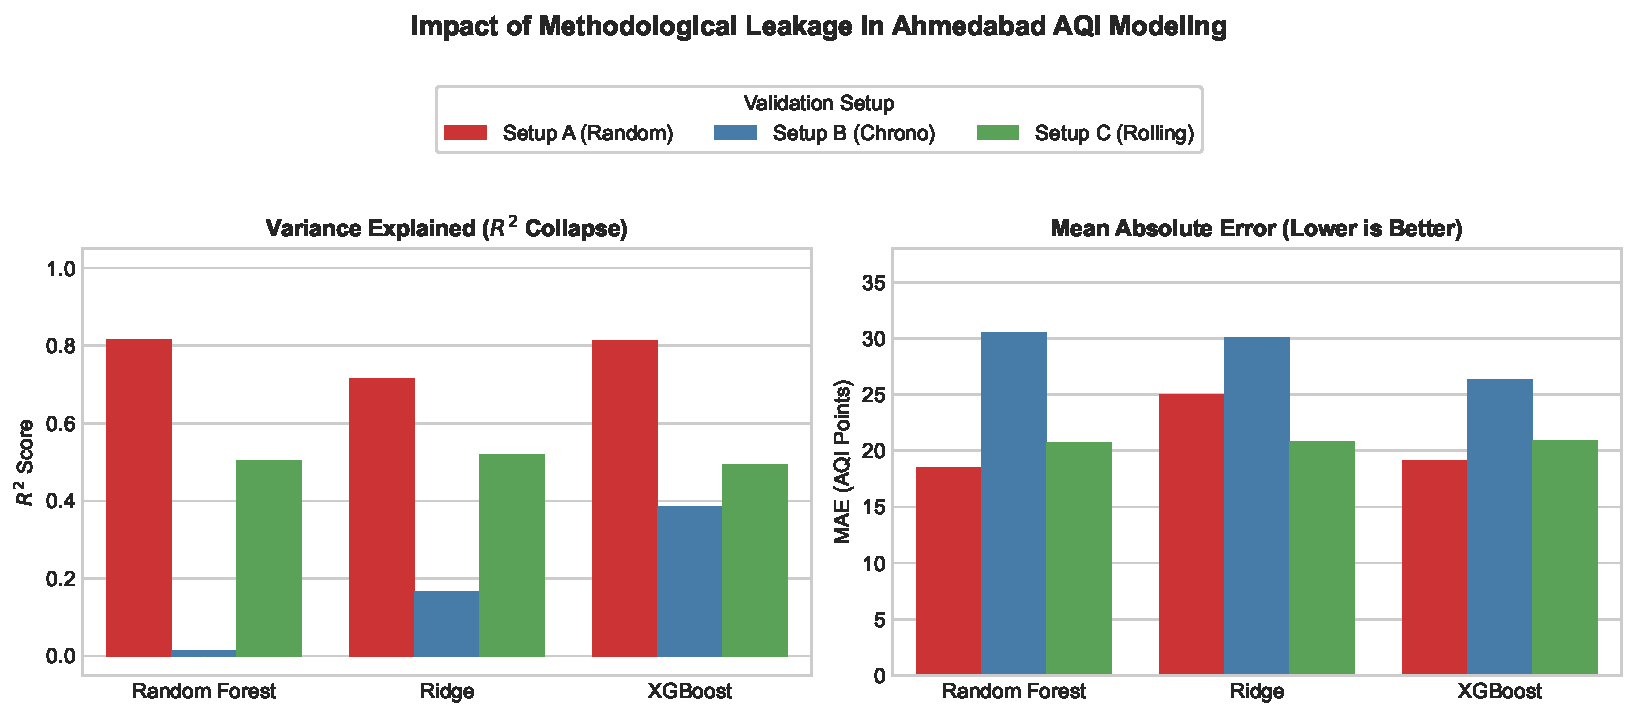
\includegraphics[width=0.88\textwidth]{../results/figures/fig1_leakage_inflation.pdf}
  \caption{Primary full-window leakage audit in Ahmedabad across Setups~A, B, and C for $R^2$ (left) and MAE (right). Lockdown-excluded Setup~A/B and like-for-like 230-day Setup~C sensitivity rows are reported in Table~\ref{tab:leakage_inflation}.}
  \label{fig:leakage_inflation}
\end{figure}

The comparison between Setup~A and Setup~B shows how strongly temporal regime shifts affect concurrent-input models. In Setup~A (random splitting with concurrent inputs, 10 seeds, $n_{\text{train}} = 919$, $n_{\text{test}} = 230$, covering only days with valid PM$_{2.5}$ observations), Random Forest achieved a mean $R^2$ of $\mathbf{0.815 \pm 0.047}$ (mean MAE $= 18.50 \pm 1.64$ across seeds). Because Setups A and B are both restricted to the 1,149 Ahmedabad days with valid PM$_{2.5}$ measurements, the Setup~B test observations have \emph{observed} (not imputed) pollutant inputs. When arranged chronologically (Setup~B, $n_{\text{train}} = 919$, $n_{\text{test}} = 230$), Random Forest dropped to $R^2 = \mathbf{0.015}$ ($\text{MAE} = 30.49$) and Ridge to $R^2 = 0.166$ ($\text{MAE} = 30.07$). Crucially, Setup~B's test window (2019-10-24 to 2020-07-01) spans India's COVID-19 lockdown (which began 25 March 2020, sharply reducing ambient AQI \cite{mahato2020}). Of the 92 calendar days in March--May 2020, 89 have valid PM$_{2.5}$ and AQI records. Excluding those 89 lockdown days restores Setup~B ($n_{\text{test}} = 141$) to $R^2 = 0.747$ ($\text{MAE} = 18.01$) for Random Forest, $R^2 = 0.665$ ($\text{MAE} = 22.01$) for Ridge, and $R^2 = 0.731$ ($\text{MAE} = 19.74$) for XGBoost. Running Setup~A on the same 1,060 non-lockdown days ($n_{\text{test}} = 212$, 10 seeds) gives $\text{MAE} = 17.61 \pm 1.15$ ($R^2 = 0.829 \pm 0.041$) for Random Forest, $22.09 \pm 0.99$ ($R^2 = 0.776 \pm 0.043$) for Ridge, and $17.99 \pm 1.11$ ($R^2 = 0.833 \pm 0.037$) for XGBoost. Thus, on non-lockdown days random-split MAE inflation is small, and the remaining $\Delta R^2$ gap is at most an upper bound because $R^2$ depends on test-set variance; the primary `0.815 -> 0.015` collapse was driven mainly by the COVID-19 lockdown regime shift.

\textbf{Like-for-like Setup B vs. C comparison:} Primary Setup~B uses $n_{\text{test}} = 230$ days (2019-10-24 to 2020-07-01), whereas primary Setup~C uses $n_{\text{test}} = 507$ days (2022-08-09 to 2023-12-30; zero overlapping dates). To provide a like-for-like concurrent-vs-lagged comparison, we also evaluated Setup~C on Setup~B's exact 230-day window (Table~\ref{tab:leakage_inflation}): Persistence achieved $\text{MAE} = 33.31$ ($R^2 = 0.131$), whereas strictly lagged Random Forest ($\text{MAE} = 37.78$), XGBoost ($38.65$), and Ridge ($41.77$) all trailed Persistence. On the 141 non-lockdown subset, concurrent-input Setup~B Random Forest ($\text{MAE} = 18.01$) strongly outperformed lagged Setup~C Random Forest ($\text{MAE} = 39.33$; Persistence $42.04$), isolating the large inflation caused by concurrent same-day pollutant inputs.

\subsection{Leak-Free Next-Day Benchmark (\texorpdfstring{$h=1$}{h=1})}
\label{sec:h1_results}
Table~\ref{tab:main_benchmark_h1} documents next-day forecasting performance under leak-free Setup~C for the two anchor cities (Ahmedabad and Chennai), including 95\% moving block-bootstrap confidence intervals, alongside model MAE distributions across all six cities (Figure~\ref{fig:model_comparison}).

\begin{table}[htbp]
\centering
\caption{Setup C Next-Day ($t+1$) Forecasting Benchmark vs Persistence Baseline. \textit{Note:} Skill score denotes normalized MAE improvement over Persistence ($1 - \text{MAE}_{\text{model}}/\text{MAE}_{\text{persistence}}$); DM $p$-value evaluates two-tailed significance vs Persistence, with asterisks ($^*$) marking $p < 0.05$ in either direction (both candidate model wins and Persistence wins).}
\label{tab:main_benchmark_h1}
\resizebox{\linewidth}{!}{\begin{tabular}{llcccccc}
\toprule
City & Model & MAE & RMSE & R2 & Skill & Band Acc (\%) & DM p-value \\
\midrule
Ahmedabad & Persistence & 20.21 & 28.83 & 0.462 & 0.000 & 75.8 & -- \\
Ahmedabad & Seasonal Naive & 26.85 & 35.95 & 0.162 & -0.328 & 70.0 & 0.000$^*$ \\
Ahmedabad & Moving Average & 20.01 & 27.10 & 0.525 & 0.010 & 76.7 & 0.766 \\
Ahmedabad & Ridge & 20.83 & 27.24 & 0.520 & -0.031 & 77.5 & 0.402 \\
Ahmedabad & Random Forest & 20.73 & 27.67 & 0.505 & -0.026 & 79.5 & 0.510 \\
Ahmedabad & XGBoost & 20.91 & 28.01 & 0.493 & -0.034 & 78.7 & 0.419 \\
Chennai & Persistence & 17.90 & 28.58 & -0.034 & 0.000 & 74.4 & -- \\
Chennai & Seasonal Naive & 23.02 & 35.78 & -0.620 & -0.286 & 67.9 & 0.000$^*$ \\
Chennai & Moving Average & 18.37 & 28.48 & -0.026 & -0.026 & 72.4 & 0.494 \\
Chennai & Ridge & 16.18 & 25.05 & 0.206 & 0.096 & 78.0 & 0.010$^*$ \\
Chennai & Random Forest & 15.84 & 24.87 & 0.218 & 0.115 & 78.0 & 0.002$^*$ \\
Chennai & XGBoost & 16.11 & 25.34 & 0.188 & 0.100 & 76.9 & 0.001$^*$ \\
\bottomrule
\end{tabular}}
\end{table}


\begin{figure}[htbp]
  \centering
  \includegraphics[width=0.88\textwidth]{../results/figures/fig2_model_comparison_h1.pdf}
  \caption{Next-day ($h=1$) MAE across models and cities under Setup~C. All machine learning models fail to significantly surpass Persistence except in coastal Chennai.}
  \label{fig:model_comparison}
\end{figure}

\paragraph{Ahmedabad.}
The naive Persistence baseline achieved an MAE of \textbf{20.21} ($R^2 = 0.462$). While the 7-day Moving Average achieved an MAE of \textbf{20.01} ($+1.0\%$ skill), this difference was statistically indistinguishable from zero ($p = 0.766$ via Diebold-Mariano). Crucially, every evaluated machine learning model (Random Forest, XGBoost, and Ridge Regression) yielded negative skill scores relative to Persistence: Random Forest attained $\text{MAE} = 20.73$ ($\text{Skill} = -0.026, p = 0.510$), Ridge attained $\text{MAE} = 20.83$ ($\text{Skill} = -0.031, p = 0.402$), and XGBoost attained $\text{MAE} = 20.91$ ($\text{Skill} = -0.034, p = 0.419$). Under the Diebold-Mariano test (no HAC correction at $h=1$, $k=0$; $p > 0.40$), none of the machine learning forecasters statistically significantly outperformed the naive Persistence baseline.

\paragraph{Chennai.}
Chennai exhibited a fundamentally different atmospheric regime. In this coastal metropolis, Persistence performed poorly ($\text{Persistence } R^2 = -0.034, \text{MAE} = 17.90$), consistent with the hypothesis that maritime circulation weakens day-to-day AQI inertia. Machine learning models established statistically significant predictive skill: Random Forest reduced MAE to \textbf{15.84} ($+11.5\%$ skill, $p = 0.002$), XGBoost achieved $\text{MAE} = 16.11$ ($+10.0\%$ skill, $p = 0.001$), and Ridge attained $\text{MAE} = 16.18$ ($+9.6\%$ skill, $p = 0.010$). Note that although the marginal 95\% block-bootstrap CIs overlap (e.g., Persistence $[15.14, 21.11]$ vs.\ Random Forest $[13.39, 18.71]$), the paired Diebold-Mariano test evaluates day-by-day loss differentials and is therefore more powerful than comparing marginal confidence intervals. Because Kaggle pollutant records end in 2020, all 28 pollutant-lag columns are imputed during Chennai's 2022--2023 test window, meaning this skill derives from AQI lags, rolling AQI statistics, and calendar harmonics alone. None of these $h=1$ Chennai results survive Bonferroni correction ($\alpha = 0.05/60 = 0.00083$) under $k=0$ (though XGBoost would survive under the $k=3$ sensitivity check at $p = 0.00075$). In a 21-column AQI-only ablation dropping the 28 pollutant-lag columns, Ahmedabad ML still failed to beat Persistence (Ridge $21.17$, RF $21.33$, XGBoost $21.24$; all $p \ge 0.168$), while Chennai retained positive skill for Ridge ($16.41, p = 0.016$) and XGBoost ($16.62, p = 0.019$), with Random Forest dropping to $16.84$ ($p = 0.087$).

\subsection{Cross-City Evaluation Across Gujarat}
\label{sec:multicity_results}
Table~\ref{tab:cross_city_mae} expands the leak-free Setup~C next-day benchmark across all six evaluated cities.

\input{../results/tables/table4_multicity.tex}

Cross-city analysis reveals three distinct operational regimes:
\begin{enumerate}
  \item \textbf{Simple-Baseline Dominance (Ahmedabad, Gandhinagar):} In urban continental Gujarat, strong day-to-day autocorrelation ($\rho_1 > 0.75$; Ahmedabad 0.75, Gandhinagar 0.83) renders simple classical baselines highly competitive, and ML models fail to outperform them. In Gandhinagar, Ridge Regression achieved $\text{MAE} = 23.43$ versus Persistence $\text{MAE} = 23.88$ ($p = 0.590$); Random Forest and XGBoost performed worse than Persistence ($p = 0.143$ and $p = 0.539$), whereas simple ARIMA(1,0,0) achieved $\text{MAE} = 22.64$ ($p = 0.0005$; Table~\ref{tab:extra_baselines}).
  \item \textbf{Persistence Superiority (Vapi):} In the chemical industrial corridor of Vapi, Persistence ($\text{MAE} = \mathbf{18.98}, R^2 = 0.813$) was \emph{statistically significantly superior} to all five candidate models at $h=1$: Seasonal Naive ($p = 7.3 \times 10^{-7}$), Moving Average ($p = 0.012$), Random Forest ($p = 7.9 \times 10^{-5}$), XGBoost ($p = 0.0009$), and Ridge ($p = 0.003$). We hypothesise that highly episodic industrial emission events create heavy-tailed spikes; models may overfit to these transient shocks during training, causing over-prediction errors on subsequent standard days.
  \item \textbf{Marginal or Data-Limited Utility (Ankleshwar, Surat):} In Ankleshwar, the 7-day Moving Average achieved a marginal advantage over Persistence ($\text{MAE} = 30.76$ vs. $33.53, p = 0.048$ under $k=0$, though this loses significance under $k=3$ at $p = 0.068$). In Surat, where the monitoring record is short ($n = 327$ valid days), high variance prevented any model from achieving statistical significance at $h=1$ ($p \ge 0.237$).
\end{enumerate}

\subsection{Multi-Step Horizon Degradation (\texorpdfstring{$h=1$ vs. $h=3$}{h=1 vs h=3})}
\label{sec:horizons_results}
Table~\ref{tab:horizon_degradation} documents error growth as the forecast lead time extends from next-day ($h=1$) to three-day ahead ($h=3$), alongside observed versus predicted trajectories in Ahmedabad (Figure~\ref{fig:forecast_trajectory}) and horizon degradation rates across all cities (Figure~\ref{fig:horizon_decay}).

\input{../results/tables/table5_horizons.tex}

\begin{table}[htbp]
\centering
\caption{Diebold--Mariano Test Results at $h=3$ Under Setup~C (Candidate vs.\ Persistence). Skill $= 1 - \text{MAE}_{\text{model}}/\text{MAE}_{\text{persistence}}$. Asterisk (*) denotes $p < 0.05$.}
\label{tab:dm_h3}
\resizebox{\linewidth}{!}{\begin{tabular}{llrrrrc}
\toprule
City & Model & MAE ($h=3$) & Persistence MAE & Skill (\%) & DM $p$ & Sig. \\
\midrule
Ahmedabad & 7-Day MA & 22.08 & 23.39 & 5.6 & 0.2011 &  \\
 & Seas. Naive & 28.44 & 23.39 & -21.6 & 0.0018 & * \\
 & Ridge & 23.27 & 23.39 & 0.5 & 0.9412 &  \\
 & Random Forest & 23.02 & 23.39 & 1.6 & 0.8250 &  \\
 & XGBoost & 22.26 & 23.39 & 4.8 & 0.4217 &  \\
Ankleshwar & 7-Day MA & 33.88 & 38.07 & 11.0 & 0.0290 & * \\
 & Seas. Naive & 43.91 & 38.07 & -15.3 & 0.1133 &  \\
 & Ridge & 34.88 & 38.07 & 8.4 & 0.1142 &  \\
 & Random Forest & 35.63 & 38.07 & 6.4 & 0.3620 &  \\
 & XGBoost & 35.17 & 38.07 & 7.6 & 0.2294 &  \\
Chennai & 7-Day MA & 19.73 & 21.87 & 9.8 & 0.0454 & * \\
 & Seas. Naive & 24.0 & 21.87 & -9.7 & 0.2156 &  \\
 & Ridge & 17.81 & 21.87 & 18.6 & 0.0006 & * \\
 & Random Forest & 18.08 & 21.87 & 17.4 & 0.0016 & * \\
 & XGBoost & 17.42 & 21.87 & 20.4 & 0.0002 & * \\
Gandhinagar & 7-Day MA & 29.7 & 30.96 & 4.1 & 0.3880 &  \\
 & Seas. Naive & 36.0 & 30.96 & -16.3 & 0.0367 & * \\
 & Ridge & 27.89 & 30.96 & 9.9 & 0.0219 & * \\
 & Random Forest & 31.21 & 30.96 & -0.8 & 0.9514 &  \\
 & XGBoost & 30.17 & 30.96 & 2.6 & 0.6304 &  \\
Surat & 7-Day MA & 46.04 & 56.61 & 18.7 & 0.0196 & * \\
 & Seas. Naive & 54.2 & 56.61 & 4.3 & 0.8802 &  \\
 & Ridge & 44.05 & 56.61 & 22.2 & 0.0237 & * \\
 & Random Forest & 47.45 & 56.61 & 16.2 & 0.1314 &  \\
 & XGBoost & 49.09 & 56.61 & 13.3 & 0.2803 &  \\
Vapi & 7-Day MA & 26.2 & 23.86 & -9.8 & 0.5396 &  \\
 & Seas. Naive & 28.94 & 23.86 & -21.3 & 0.1547 &  \\
 & Ridge & 26.09 & 23.86 & -9.4 & 0.7127 &  \\
 & Random Forest & 28.75 & 23.86 & -20.5 & 0.2260 &  \\
 & XGBoost & 28.68 & 23.86 & -20.2 & 0.1862 &  \\
\bottomrule
\end{tabular}}
\end{table}

\begin{figure}[htbp]
  \centering
  \includegraphics[width=0.88\textwidth]{../results/figures/fig3_forecast_trajectory.pdf}
  \caption{Next-day predicted versus observed AQI trajectories for Ahmedabad over a 90-day operational test window under Setup~C.}
  \label{fig:forecast_trajectory}
\end{figure}

\begin{figure}[htbp]
  \centering
  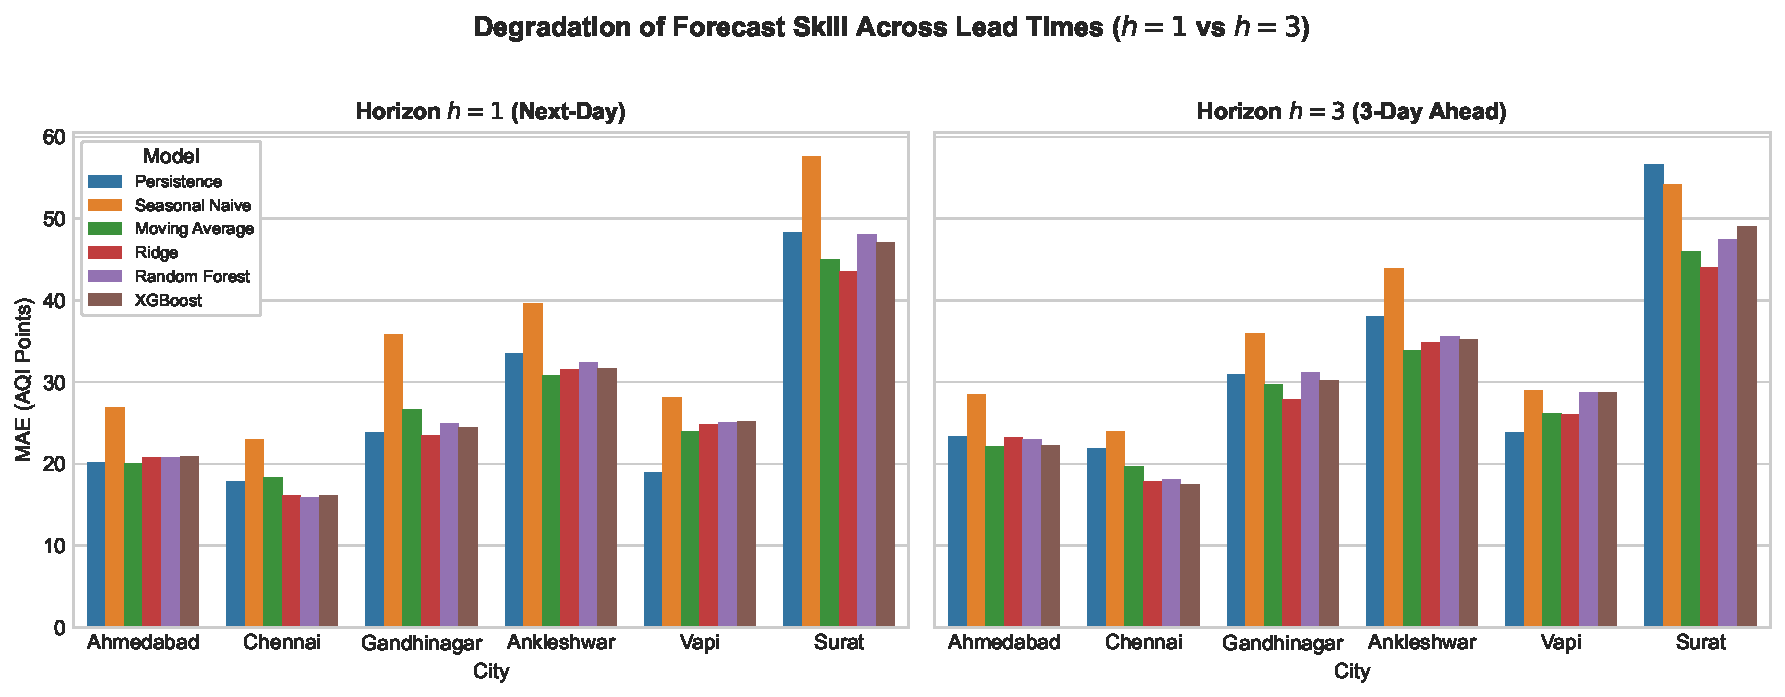
\includegraphics[width=0.88\textwidth]{../results/figures/fig5_horizon_decay.pdf}
  \caption{Horizon degradation from $h=1$ to $h=3$ across cities under Setup~C. Persistence error increases faster than multi-lag linear and moving-average models.}
  \label{fig:horizon_decay}
\end{figure}

As the forecast horizon extends to $h=3$, the predictive power of single-step persistence decays rapidly: in Gandhinagar, Persistence MAE degrades by $+29.6\%$ (from $23.88$ to $30.96$); in Vapi, it degrades by $+25.7\%$ (from $18.98$ to $23.86$). The 7-Day Moving Average and Seasonal Naive degrade by $-6\%$ to $+12\%$ (Surat Seasonal Naive even improves by $-6.0\%$). Ridge Regression degrades by $+1\%$ to $+19\%$, with Gandhinagar Ridge the worst case at $+19.0\%$. Tree ensembles span $-1\%$ to $+25\%$ (Surat Random Forest $-1.4\%$ to Gandhinagar Random Forest $+24.9\%$).

Consequently, machine learning models demonstrate nominally significant utility at extended lead times: in Gandhinagar at $h=3$, Ridge Regression achieved an MAE of \textbf{27.89} versus Persistence \textbf{30.96} ($+9.9\%$ skill, $p = 0.022$, Table~\ref{tab:dm_h3}); in Surat at $h=3$, Ridge achieved $\text{MAE} = \mathbf{44.05}$ versus Persistence \textbf{56.61} ($+22.2\%$ skill, $p = 0.024$, Table~\ref{tab:dm_h3}); and in Chennai the 7-Day Moving Average also reached significance ($p = 0.045$). However, only Chennai Ridge ($p = 0.0006$) and XGBoost ($p = 0.0002$) survive Bonferroni correction at $h=3$; Chennai Random Forest ($p = 0.0016$), Gandhinagar Ridge ($p = 0.022$), and Surat Ridge ($p = 0.024$) do not. Bonferroni-corrected skill is therefore confirmed only for Chennai at $h=3$. Moreover, at $h=3$ in Chennai, ARIMA(1,0,0) achieved $\text{MAE} = 21.13$ (no better than Persistence $21.87$, $p = 0.531$), whereas all three Chennai ML models significantly outperformed ARIMA(1,0,0) (Ridge $p = 0.0001$, Random Forest $p = 0.0009$, XGBoost $p < 0.0001$). Full $h=3$ Diebold-Mariano results for all cities and models are reported in Table~\ref{tab:dm_h3}.

\subsection{Diebold-Mariano Test Synthesis}
\label{sec:dm_synthesis}
The Diebold-Mariano $p$-values across all evaluated city and model configurations at $h=1$ under Setup~C are summarised in a heatmap (Figure~\ref{fig:diebold_mariano}), while full $h=3$ results appear in Table~\ref{tab:dm_h3}.

\begin{figure}[htbp]
  \centering
  \includegraphics[width=0.88\textwidth]{../results/figures/fig4_diebold_mariano.pdf}
  \caption{Diebold-Mariano test $p$-values comparing candidate forecasters to Persistence under Setup~C ($h=1$). Darker blue indicates smaller two-tailed $p$-values ($p < 0.05$ in either direction, i.e., either candidate superiority or Persistence dominance); lighter yellow indicates non-significant differences.}
  \label{fig:diebold_mariano}
\end{figure}

Across 60 pairwise comparisons (6 cities $\times$ 5 candidate models $\times$ 2 horizons), 12 configurations establish statistically significant differences ($p < 0.05$) in favour of the candidate model: 4 at $h=1$ (Ankleshwar Moving Average $p = 0.048$, and Chennai Ridge $p = 0.010$, Random Forest $p = 0.002$, and XGBoost $p = 0.001$) and 8 at $h=3$ (Ankleshwar Moving Average $p = 0.029$; Chennai Moving Average $p = 0.045$, Ridge $p = 0.0006$, Random Forest $p = 0.0016$, and XGBoost $p = 0.0002$; Gandhinagar Ridge $p = 0.022$; and Surat Moving Average $p = 0.020$ and Ridge $p = 0.024$; full $h=3$ breakdown in Table~\ref{tab:dm_h3}). Conversely, Persistence is statistically superior to candidate models in 12 configurations (10 at $h=1$ and 2 at $h=3$). In Vapi at $h=1$, Persistence outperforms all five candidate models: Seasonal Naive ($p = 7.3 \times 10^{-7}$), Moving Average ($p = 0.012$), Ridge ($p = 0.003$), XGBoost ($p = 0.0009$), and Random Forest ($p = 7.9 \times 10^{-5}$). Beyond Vapi, Persistence also beats Seasonal Naive in Ahmedabad ($p = 9.3 \times 10^{-9}$), Chennai ($p = 2.5 \times 10^{-6}$), Gandhinagar ($p = 5.1 \times 10^{-11}$), and Ankleshwar ($p = 0.015$), beats Moving Average in Gandhinagar ($p = 0.019$), and beats Seasonal Naive at $h=3$ in Ahmedabad ($p = 0.002$) and Gandhinagar ($p = 0.037$). Applying a conservative Bonferroni correction for the primary family of 60 candidate-vs-Persistence comparisons ($\alpha = 0.05 / 60 = 0.00083$), only 2 candidate wins survive (Chennai Ridge $p = 0.0006$ and XGBoost $p = 0.0002$ at $h=3$; Chennai ML models at $h=1$ under $k=0$ and Chennai Random Forest at $h=3$ do \emph{not} survive), while 5 Persistence wins survive under $k=0$ (Vapi Random Forest $p = 7.9 \times 10^{-5}$ and Seasonal Naive $p = 7.3 \times 10^{-7}$, plus Seasonal Naive in Ahmedabad, Chennai, and Gandhinagar; Vapi XGBoost at $p = 0.0009$ does \emph{not} survive, and the 5-win count depends on $k=0$ since Vapi Random Forest shifts to $p = 0.0058$ under $k=3$).

\textit{Note on DM bandwidth and sensitivity:} At $h=1$, the lag truncation is $k = h - 1 = 0$, meaning no autocorrelation correction is applied to the loss-differential variance; the DM test at $h=1$ reduces to a Harvey--Leybourne--Newbold small-sample corrected $t$-test on the loss differentials. At $h=3$, $k=2$ lags are used. To verify that our $h=1$ conclusions are not artefacts of $k=0$, we re-ran the DM test with lag truncation $k=3$ across all six cities. In Chennai, all three ML models remained statistically significant (Ridge $p = 0.008$, Random Forest $p = 0.0018$, and XGBoost $p = 0.00075$, which would survive the 0.00083 Bonferroni threshold under $k=3$); in Vapi, Persistence remained statistically superior to all ML models (Random Forest $p = 0.0058$, XGBoost $p = 0.0085$, Ridge $p = 0.038$), while Ankleshwar Moving Average ($p = 0.068$) and Gandhinagar Moving Average ($p = 0.069$) lost nominal significance.

\paragraph{Additional Baselines and Tuned-Model Sensitivity Check.}
Table~\ref{tab:extra_baselines} reports all four supplementary classical baselines (Climatology, Climatology+Persistence, ARIMA(1,0,0), and ETS) across all six cities under Setup~C ($h=1$).

\begin{table}[htbp]
\centering
\caption{Additional Classical Baselines at $h=1$ Under Setup~C (MAE, Skill vs.\ Persistence, and Two-Tailed DM $p$-Value). Asterisk ($^*$) denotes $p < 0.05$ in either direction (candidate win or Persistence win).}
\label{tab:extra_baselines}
\resizebox{0.9\linewidth}{!}{\begin{tabular}{llrrrc}
\toprule
City & Baseline & MAE & Pers.\ MAE & Skill & DM $p$-value \\
\midrule
Ahmedabad & Climatology & 34.70 & 20.21 & -0.717 & $<$0.0001$^*$ \\
 & Clim. + Pers. & 23.28 & 20.21 & -0.152 & 0.0002$^*$ \\
 & ARIMA(1,0,0) & 21.41 & 20.21 & -0.059 & 0.0177$^*$ \\
 & ETS (SES) & 27.63 & 20.21 & -0.367 & $<$0.0001$^*$ \\
Ankleshwar & Climatology & 39.24 & 33.53 & -0.171 & 0.0151$^*$ \\
 & Clim. + Pers. & 32.04 & 33.53 & +0.044 & 0.1047 \\
 & ARIMA(1,0,0) & 34.04 & 33.53 & -0.015 & 0.0115$^*$ \\
 & ETS (SES) & 35.60 & 33.53 & -0.062 & 0.6941 \\
Chennai & Climatology & 22.38 & 17.90 & -0.251 & $<$0.0001$^*$ \\
 & Clim. + Pers. & 17.25 & 17.90 & +0.036 & 0.1366 \\
 & ARIMA(1,0,0) & 16.96 & 17.90 & +0.052 & 0.0035$^*$ \\
 & ETS (SES) & 17.85 & 17.90 & +0.003 & 0.8198 \\
Gandhinagar & Climatology & 30.32 & 23.88 & -0.270 & $<$0.0001$^*$ \\
 & Clim. + Pers. & 22.44 & 23.88 & +0.060 & 0.1216 \\
 & ARIMA(1,0,0) & 22.64 & 23.88 & +0.052 & 0.0005$^*$ \\
 & ETS (SES) & 22.47 & 23.88 & +0.059 & 0.0460$^*$ \\
Surat & Climatology & 56.57 & 48.26 & -0.172 & 0.2542 \\
 & Clim. + Pers. & 45.56 & 48.26 & +0.056 & 0.1311 \\
 & ARIMA(1,0,0) & 42.13 & 48.26 & +0.127 & 0.0106$^*$ \\
 & ETS (SES) & 41.27 & 48.26 & +0.145 & 0.1501 \\
Vapi & Climatology & 39.94 & 18.98 & -1.104 & $<$0.0001$^*$ \\
 & Clim. + Pers. & 27.94 & 18.98 & -0.472 & $<$0.0001$^*$ \\
 & ARIMA(1,0,0) & 25.23 & 18.98 & -0.329 & 0.2915 \\
 & ETS (SES) & 31.42 & 18.98 & -0.656 & $<$0.0001$^*$ \\
\bottomrule
\end{tabular}}
\end{table}

Monthly Climatology performed substantially worse than Persistence in every city (all $p \le 0.0151$ except Surat $p = 0.254$), and Climatology+Persistence never significantly beat Persistence ($p \ge 0.105$ where its MAE was lower; it was significantly worse in Ahmedabad, $p = 0.0002$, and Vapi, $p < 0.0001$). ARIMA(1,0,0) and ETS failed to beat Persistence in Ahmedabad (ARIMA MAE $21.41, p = 0.018$; ETS $27.63, p < 0.0001$), Ankleshwar, and Vapi, while ETS gained significantly in Gandhinagar ($\text{MAE} = 22.47, p = 0.046$) and ARIMA(1,0,0) achieved statistically significant gains in Gandhinagar ($\text{MAE} = 22.64, p = 0.0005$, surviving even an 80-test Bonferroni threshold of $0.000625$), Surat ($\text{MAE} = 42.13, p = 0.011$), and Chennai ($\text{MAE} = 16.96, p = 0.0035$). In Gandhinagar and Surat, simple ARIMA(1,0,0) achieved lower MAE than every ML model in Table~\ref{tab:cross_city_mae}. Direct DM tests comparing ML against ARIMA(1,0,0) at $h=1$ show that in Gandhinagar ARIMA(1,0,0) significantly outperformed Random Forest ($p = 0.0022$) and XGBoost ($p = 0.0339$; vs.\ Ridge $p = 0.287$); in Surat differences were non-significant ($p \ge 0.228$); and in Chennai only Random Forest ($15.84$ vs.\ $16.96, p = 0.030$) significantly beat ARIMA(1,0,0) (Ridge $p = 0.112$, XGBoost $p = 0.064$). Finally, tuning hyperparameters on Ahmedabad via 3-fold \texttt{TimeSeriesSplit} on the initial training fold yielded Ridge ($\alpha=500$: MAE $21.03, p = 0.303$), Random Forest (\texttt{max\_depth=5, min\_samples\_leaf=5, n\_estimators=200}: MAE $20.22, p = 0.955$), and XGBoost (\texttt{lr=0.05, max\_depth=2, n\_estimators=200}: MAE $19.99, p = 0.734$). None significantly outperformed Persistence ($20.21$), confirming that ML underperformance in inland Gujarat is not an artefact of fixed default hyperparameters.


%% ════════════════════════════════════════════════════════════════════════════
\section{Discussion}
\label{sec:discussion}

\subsection{Why Are Simple Baselines Hard to Beat in Gujarat?}
The empirical finding that complex machine learning algorithms fail to surpass simple classical baselines (with Persistence the simplest, and ARIMA(1,0,0) achieving lower MAE than or outperforming ML in Gandhinagar and Surat) across continental Gujarat is consistent with atmospheric persistence in these regions. In inland, semi-arid regions characterised by stable anticyclonic synoptic conditions during autumn and winter, daily boundary layer dynamics, nocturnal temperature inversions, and local anthropogenic emissions exhibit high day-to-day inertia. We hypothesise that because the atmospheric system changes gradually, yesterday's 24-hour mean AQI represents a near-sufficient statistic for tomorrow's mean state under unperturbed conditions. Machine learning models trained on purely lagged surface concentrations cannot anticipate external synoptic shifts without numerical meteorological forcing.

\subsection{The Coastal Exception: Dynamics of Chennai}
In contrast, Chennai's maritime boundary layer is governed by diurnal mesoscale land-sea breeze circulations and maritime moisture advection. These dynamics may reduce day-to-day AQI inertia, creating structured periodic patterns that cyclical calendar harmonics and autoregressive AQI patterns can exploit (noting that Chennai's 2022--2023 test window has imputed pollutant lags). This may explain why machine learning models achieved nominally significant $+11.5\%$ skill improvements in Chennai while failing to beat persistence in Ahmedabad and Gandhinagar; we treat this as a working hypothesis pending residual analysis with meteorological covariates.

\subsection{Overfitting to Industrial Emissions: The Case of Vapi}
The statistically significant underperformance of Random Forest and XGBoost in Vapi ($p \leq 0.003$ relative to Persistence) highlights a critical vulnerability in applied environmental machine learning. Vapi is an intensive chemical manufacturing hub subject to sporadic, unannounced industrial batch releases. These intermittent emissions produce heavy-tailed spikes in criteria pollutants. We hypothesise that nonlinear tree ensembles may branch heavily on these high-magnitude anomalies during training, learning spurious split boundaries. When ambient conditions revert to typical baselines, these models project lingering elevations, producing substantial over-prediction errors. Simple persistence, which tracks only the immediate preceding state, avoids this structural over-prediction.

\subsection{Recommendations for Environmental Data Science}
Based on our findings, we propose four methodological standards for atmospheric machine learning studies:
\begin{enumerate}
  \item \textbf{Persistence and AR(1) Benchmarking:} Every urban AQI forecasting study should include the naive Persistence baseline ($\hat{y}_{t+h} = y_t$) and a simple AR(1) benchmark, reporting relative forecast skill scores rather than raw accuracy metrics alone.
  \item \textbf{Avoid Random Splitting:} Random train-test partitioning should not be used on environmental time series. Evaluations should enforce temporal separation via rolling-origin or blocked prequential protocols.
  \item \textbf{Exclusion of Concurrent Pollutants from Forecasting Benchmarks:} Predictor matrices should exclude same-day criteria pollutant concentrations unless the task is explicitly framed as algebraic reconstruction or nowcasting.
  \item \textbf{Formal Statistical Significance Testing:} Authors should conduct formal hypothesis tests (e.g., Diebold-Mariano with HAC variance estimators) to substantiate claims of algorithmic superiority.
\end{enumerate}

\subsection{Limitations}
\label{sec:limitations}
Several limitations of the present study should be noted:
\begin{itemize}
  \item \textbf{Station Network Heterogeneity:} City-level AQI values represent spatial averages across active municipal CAAQMS stations. Station additions or maintenance outages over the 2015--2023 timeframe may introduce minor unmodelled level shifts in the aggregate series.
  \item \textbf{Exclusion of Numerical Weather Prediction (NWP) Forcing:} To isolate the autoregressive information content of surface monitoring records, this benchmark excluded numerical weather forecasts (wind vector, mixing height, relative humidity). Incorporating high-resolution operational NWP grids represents an essential avenue for future research.
  \item \textbf{Fixed Hyperparameter Regimes:} Primary benchmark hyperparameters were held constant across cities to prevent post-hoc optimization leakage. While a 3-fold \texttt{TimeSeriesSplit} tuned check on Ahmedabad yielded no significant improvement over Persistence ($\text{MAE} = 19.99\text{--}21.03$, all $p \ge 0.30$), full nested rolling-origin tuning across all cities could yield marginal refinements.
  \item \textbf{Pollutant Coverage and Regime Shifts:} Kaggle pollutant records end in 2020, so training folds in Ahmedabad and Chennai contain observed 2015--2020 pollutant lags whereas their 2022--2023 Setup~C test inputs are imputed. A 21-column AQI-only ablation confirms that Ahmedabad ML still fails to beat Persistence ($\text{MAE} = 21.17\text{--}21.33$, $p \ge 0.168$), while in Chennai Random Forest drops from $15.84$ ($p = 0.002$) to $16.84$ ($p = 0.087$). Similarly, Setup~B's test window overlaps the March--May 2020 COVID-19 lockdown regime shift, which accounts for most of its apparent $R^2$ collapse.
  \item \textbf{Geographical Scope:} Our empirical scope centered on western India (Gujarat) and a southern maritime anchor (Chennai). Extending this audit to the Indo-Gangetic Plain, where intense seasonal biomass burning and winter fog inversions prevail, constitutes an important next step.
\end{itemize}


%% ════════════════════════════════════════════════════════════════════════════
\section{Conclusion}
\label{sec:conclusion}

This paper presented an empirical audit of data leakage in Indian air quality forecasting literature and established, to our knowledge, the first leak-free, rolling-origin benchmark across Gujarat cities. We demonstrated that the combination of concurrent pollutant inputs, random train-test splitting, and temporal regime shifts can produce severe apparent performance inflation -- exemplified by Random Forest in Ahmedabad, where explained variance ($R^2$) fell from $0.815$ under Setup~A to $0.015$ under Setup~B (though excluding the March--May 2020 COVID-19 lockdown days from Setup~B restores $R^2$ to $0.747$, showing that distribution shift contributed substantially alongside autocorrelation leakage).

Under rigorous, leak-free rolling-origin evaluation at next-day lead times ($h=1$), machine learning models failed to statistically outperform simple classical baselines (with Persistence the simplest, and ARIMA(1,0,0) matching or beating ML in Gandhinagar and Surat) in five of six evaluated cities. In industrial Vapi, Persistence was itself statistically superior to Random Forest and XGBoost ($p \leq 0.003$). At $h=1$, machine learning established nominally significant skill only in coastal Chennai ($+11.5\%$ skill, $p = 0.002$), though this does not survive Bonferroni correction under $k=0$ ($\alpha = 0.05/60$; XGBoost is borderline at $p = 0.00075$ under $k=3$). Genuine Bonferroni-corrected skill is confirmed at multi-day lead times ($h=3$) in Chennai (Ridge $p = 0.0006$, XGBoost $p = 0.0002$) where atmospheric autocorrelation naturally attenuates.

These findings demonstrate that future research claiming algorithmic superiority for urban air quality forecasting should benchmark against persistence under strict temporal validation. To support community adoption, our complete pipeline, datasets, and evaluation ledgers are openly accessible.

%% ════════════════════════════════════════════════════════════════════════════
\section*{Acknowledgements}
The author acknowledges the Central Pollution Control Board (CPCB), Ministry of Environment, Forest and Climate Change, Government of India, for maintaining the public air quality monitoring network and making municipal bulletin records publicly accessible.

\section*{Reproducibility Statement}
The entire experimental pipeline is designed for full, single-command reproduction. Source code, configuration files, cleaned datasets, and pre-computed prediction ledgers are openly accessible at: \url{https://github.com/Pratham1227-beep/aqi-gujarat-leakage}. Complete execution commands, dependencies, and reproduction instructions are provided in the repository README.

%% ════════════════════════════════════════════════════════════════════════════


%% References (IEEE / Numeric Style)
%% ════════════════════════════════════════════════════════════════════════════
\begin{thebibliography}{99}
\small

\bibitem{pandey2021}
A.~Pandey et al., ``Health and economic impact of air pollution in the states of India: The Global Burden of Disease Study 2019,'' \emph{The Lancet Planetary Health}, vol.~5, no.~1, pp.~e25--e38, 2021.

\bibitem{gulia2015}
S.~Gulia, S.~M.~Shiva Nagendra, M.~Khare, and I.~Khanna, ``Urban air quality management -- a review,'' \emph{Atmospheric Pollution Research}, vol.~6, no.~2, pp.~286--304, 2015.

\bibitem{maltare2023}
N.~N.~Maltare and S.~A.~Vahora, ``Air quality index prediction using machine learning for Ahmedabad city,'' \emph{Digital Chemical Engineering}, vol.~7, p.~100093, 2023.

\bibitem{advitha2024}
G.~Advitha, A.~N.~Varaprasad, K.~V.~Khushi, P.~Vijay, and S.~Nayak, ``Cultivating clean skies: Unveiling the tapestry of air quality in Gujarat through innovative machine learning analysis,'' \emph{Big Data and Computing Visions}, vol.~4, no.~4, pp.~326--339, 2024, doi: 10.22105/bdcv.2024.485515.1213.

\bibitem{sidhu2024}
K.~K.~Sidhu, H.~Balogun, and K.~O.~Oseni, ``Predictive modelling of Air Quality Index (AQI) across diverse cities and states of India using machine learning: Investigating the influence of Punjab's stubble burning on AQI variability,'' \emph{International Journal of Management and Information Technology}, vol.~16, no.~1, 2024. (arXiv:2404.08702).

\bibitem{mishra2025}
D.~Mishra, A.~Sahu, and S.~Naman, ``Implementation of boosting algorithms in predicting air quality index of South Indian cities,'' \emph{Engineering Innovations}, vol.~14, pp.~99--115, 2025.

\bibitem{jayapradha2025}
J.~Jayapradha, S.-C.~Haw, N.~Palanichamy, V.~Arunesh, S.~Pranav, and T.~S.~Kumar, ``LRX: A hybrid-based real-time air quality index prediction and visualization model,'' \emph{Emerging Science Journal}, vol.~9, no.~5, pp.~2454--2470, 2025.
\bibitem{chauhan2026}
K.~Chauhan and K.~Sutaria, ``Machine learning-based air quality monitoring in Indian metropolitan cities: A comparative study,'' \emph{International Journal of Advanced Computer Science and Applications (IJACSA)}, vol.~17, no.~3, 2026.

\bibitem{chakraborty2026}
P.~Chakraborty and Shanthi~P.~B., ``A dual-branch explainable AI framework combining machine and deep learning for air quality forecasting in Indian cities,'' \emph{Research Square Preprint}, 2026. [Online]. Available: \url{https://www.researchsquare.com/article/rs-8956323/v1}

\bibitem{singh2025}
S.~K.~Singh, R.~Jain, D.~Palaniappan, K.~Parmar, Premavathi~T., and J.~Gothania, ``Spatiotemporal analysis and machine learning-based prediction of air quality in Indian urban cities,'' \emph{Environmental Research and Technology}, vol.~8, no.~4, pp.~809--822, 2025.

\bibitem{malhotra2024}
M.~Malhotra, S.~Walia, C.-C.~Lin, I.~K.~Aulakh, and S.~Agarwal, ``A systematic scrutiny of artificial intelligence-based air pollution prediction techniques, challenges, and viable solutions,'' \emph{Journal of Big Data}, vol.~11, 2024, doi: 10.1186/s40537-024-01002-8.

\bibitem{mahendra2023}
H.~N.~Mahendra, S.~Mallikarjunaswamy, D.~M.~Kumar, S.~Kumari, S.~Kashyap, S.~Fulwani, and A.~Chatterjee, ``Assessment and prediction of air quality level using ARIMA model: A case study of Surat city, Gujarat State, India,'' \emph{Nature Environment and Pollution Technology}, vol.~22, no.~1, pp.~199--210, 2023, doi: 10.46488/nept.2023.v22i01.018.

\bibitem{goetzinger2026}
P.~Goetzinger, S.~Noy, and K.~Huffstadt, ``Machine learning approaches for predicting air pollution levels: A transparent, time-aware pipeline for daily AQI in Indian cities,'' \emph{Modeling Earth Systems and Environment}, vol.~12, no.~2, art.~no.~97, 2026, doi: 10.1007/s40808-026-02741-8.

\bibitem{dar2025}
A.~A.~Dar and A.~J.~Shaik, ``Spatiotemporal clustering and multivariate forecasting of air quality index across Indian cities using machine learning and deep learning models,'' \emph{Franklin Open}, vol.~13, art.~no.~100435, 2025, doi: 10.1016/j.fraope.2025.100435.

\bibitem{abidha2026}
A.~K.~Abidha, S.~J.~Kumaar, A.~A.~Dar, and M.~S.~Khan, ``Leakage-aware explainable air quality index forecasting in urban environments using machine learning and time series models: A case study of Chennai, India,'' \emph{Ing{\'e}nierie des Syst{\`e}mes d'Information (IIETA)}, vol.~31, no.~9, pp.~2963--2974, 2026, doi: 10.18280/isi.310907.

\bibitem{ayus2023}
I.~Ayus, N.~Natarajan, and D.~Gupta, ``Comparison of machine learning and deep learning techniques for the prediction of air pollution: A case study from China,'' \emph{Asian Journal of Atmospheric Environment}, vol.~17, art.~no.~4, 2023.

\bibitem{kaufman2012}
S.~Kaufman, S.~Rosset, C.~Perlich, and O.~Stitelman, ``Leakage in data mining: Formulation, detection, and avoidance,'' \emph{ACM Transactions on Knowledge Discovery from Data}, vol.~6, no.~4, pp.~1--21, 2012.

\bibitem{bergmeir2012}
C.~Bergmeir and J.~M.~Ben{\'i}tez, ``On the use of cross-validation for time series predictor evaluation,'' \emph{Information Sciences}, vol.~191, pp.~192--213, 2012.

\bibitem{cerqueira2020}
V.~Cerqueira, L.~Torgo, and I.~Mozeti{\v{c}}, ``Evaluating time series forecasting models: An empirical study on performance estimation methods,'' \emph{Machine Learning}, vol.~109, no.~11, pp.~1997--2028, 2020.

\bibitem{murphy1992}
A.~H.~Murphy, ``Climatology, persistence, and their linear combination as standards of reference in skill scores,'' \emph{Weather and Forecasting}, vol.~7, no.~4, pp.~692--698, 1992.

\bibitem{jolliffe2012}
I.~T.~Jolliffe and D.~B.~Stephenson, Eds., \emph{Forecast Verification: A Practitioner's Guide in Atmospheric Science}, 2nd ed. Chichester, U.K.: Wiley, 2012.

\bibitem{albelali2025}
S.~Albelali and M.~Ahmed, ``Hidden leaks in time series forecasting: How data leakage affects LSTM evaluation across configurations and validation strategies,'' arXiv preprint arXiv:2512.06932, 2025.

\bibitem{garciacrespi2026}
F.~Garc{\'i}a Crespi, E.~Yubero Funes, and M.~Alfosea Sim{\'o}n, ``Rolling-origin validation reverses model rankings in multi-step PM$_{10}$ forecasting: XGBoost, SARIMA, and persistence,'' arXiv preprint arXiv:2603.20315, 2026.

\bibitem{xie2025}
Y.~Xie and S.~P.~Tummala, ``Machine learning for sensor analytics: A comprehensive review and benchmark of boosting algorithms in healthcare, environmental, and energy applications,'' \emph{Sensors}, vol.~25, no.~23, art.~no.~7294, 2025, doi: 10.3390/s25237294.

\bibitem{diebold1995}
F.~X.~Diebold and R.~S.~Mariano, ``Comparing predictive accuracy,'' \emph{Journal of Business \& Economic Statistics}, vol.~13, no.~3, pp.~253--263, 1995.

\end{thebibliography}

\end{document}
